\documentclass[man]{apa}
\usepackage{graphicx,epsfig,amsmath,alltt,setspace,bm}
\title{Studying measurement invariance in factor analysis models
  via stochastic processes}
\twoauthors{Edgar C. Merkle}{Achim Zeileis}
\twoaffiliations{Wichita State University}{Universit\"{a}t Innsbruck}

\abstract{The issue of measurement invariance commonly arises in
  factor-analytic contexts, with methods for assessment
  including 
  likelihood ratio tests, Lagrange multiplier tests, and
  Wald tests.  These tests all require advance definition of the number of
  groups, group 
  membership, and offending model parameters.
In this paper, we construct tests of parameter
invariance based on stochastic processes of casewise
derivatives of the likelihood function.  These tests can be viewed as
generalizations of the Lagrange multiplier test, and they are especially
useful for: (1) isolating specific parameters affected by measurement
invariance violations, and (2) identifying subgroups of individuals
that violated measurement invariance based on a continuous auxiliary
variable.  The tests are presented and illustrated in detail, along
with simulations examining the tests' abilities in controlled conditions.}

\acknowledgements{Correspondence to Edgar C.\
  Merkle, Department of 
  Psychology, Wichita State University, Wichita, KS 67260-0034.
  Email: {\texttt{edgar.merkle@wichita.edu}}.}
\shorttitle{Parameter instability tests}
\rightheader{Parameter instability tests}

\newcommand{\argmax}{\operatorname{argmax}\displaylimits}

%% for internal use
\newcommand{\fixme}[1]{\emph{\marginpar{FIXME} (#1)}}
\newcommand{\readme}[1]{\emph{\marginpar{README} (#1)}}

\begin{document}
\maketitle

The assumption that parameters are
invariant across observations is a
fundamental tenet of many statistical models.  A specific type of 
parameter invariance, measurement invariance, has implications for the
general design and use of psychometric scales.
This concept is 
particularly important because violations can render the scales
useless.  
That is, if a set of scales violates measurement invariance,
then individuals with the same ``amount'' of a latent variable 
may systematically receive 
different scale scores.
This may lead researchers to conclude subgroup
differences on a wide variety of interesting constructs 
when, in reality, the scales are the sole cause of the 
differences.  Further, it can be inappropriate to incorporate scales
violating measurement invariance into structural equation
models, where relationships between constructs are hypothesized.  Horn
and McArdle \citeyear{HorMca92} concisely summarize the impact of
these issues, stating ``Lack of evidence of measurement 
invariance equivocates conclusions and casts doubt on theory in the
behavioral sciences'' (p.\ 141).  Borsboom \citeyear{Bor06a} also
notes that researchers often fail to assess whether measurement
invariance holds.

In this paper, we consider a new family of tests for assessing
measurement invariance that have important advantages over existing
tests.  We begin by developing a general framework for the tests.
This leads to a discussion of theoretical results relevant to the
proposed tests, as well as a comparison of the proposed tests with
existing tests.  Next,
we study the 
proposed tests' abilities through example and simulation.  Finally,
we discuss some interesting extensions of the tests.
Throughout the manuscript, we use the term {\em{test}} to refer to a
statistical test and the term {\em{scale}} to refer to a psychometric 
test or scale.

\section{Framework}

The methods proposed here are generally relevant to situations where the
$p$-dimensional random variable $X$ with associated observations $\bm{x}_i, i=1,\cdots,n$
is specified to arise from a model with density $f(\bm{x}_i; \bm{\theta})$ and
associated joint log-likelihood
\begin{equation} \label{eq:loglik}
  \ell(\bm{\theta}; \bm{x}_1, \dots, \bm{x}_n) ~=~
    \sum_{i = 1}^n \ell(\bm{\theta}; \bm{x}_i) ~=~
    \sum_{i = 1}^n  \log f(\bm{x}_i; \bm{\theta}),
\end{equation}
where ${\bm \theta}$ is some $k$-dimensional parameter vector that characterizes
the distribution. 
The methods are applicable under very general conditions, essentially
whenever standard assumptions for maximum likelihood inference hold (for more
details see below). For empirical applications, we employ
a specific factor analysis model where the data follow a multivariate normal
distribution:
\begin{eqnarray}
    \label{eq:mvndensity}
    f(\bm{x}_i; \bm{\theta}) & = & \frac{1}{(2\pi)^{p/2} |
      \bm{\Sigma}(\bm{\theta}) |^{1/2}} ~ \exp \left\{ -\frac{1}{2}(\bm{x}_i -
    \bm{\mu}(\bm{\theta}))^{\top} \bm{\Sigma}(\bm{\theta})^{-1} (\bm{x}_i -
    \bm{\mu}(\bm{\theta}) \right\}, \\
    \label{eq:caselik}
    \ell(\bm{\theta}; \bm{x}_i) & = & -\frac{1}{2} \left\{
      (\bm{x}_i - \bm{\mu}(\bm{\theta}))^{\top} \bm{\Sigma}(\bm{\theta})^{-1} (\bm{x}_i - \bm{\mu}(\bm{\theta}))
      ~+~ \log | \bm{\Sigma}(\bm{\theta}) | ~+~ p \log(2 \pi) \right\}.
\end{eqnarray}
with model-implied mean vector ${\bm{\mu}}({\bm{\theta}})$ and
covariance matrix ${\bm{\Sigma}}({\bm{\theta}})$. As pointed out above,
the assumptions for the tests introduced below do not require this specific
form of the likelihood but it is presented for illustration due to
its importance in practice.  Many expositions of factor analysis
utilize the likelihood for the sample covariance matrix, which is
based on a Wishart distribution when $\bm{x}_i$ are assumed to be
multivariate normal.
However, the techniques presented below require the casewise contributions
to the likelihood; this situation is also generally
encountered in structural equation models with missing data (e.g.,
\citeNP{Wot00}).

Within the general framework outlined above, and under the usual
regularity conditions, the model parameters $\bm{\theta}$ can
be estimated by maximum likelihood (ML), i.e.,
\begin{equation} \label{eq:ml}
  \hat{\bm{\theta}} ~=~ \argmax_{\bm{\theta}} \ell(\bm{\theta}; x_1, \dots, x_n),
\end{equation}
or equivalently by solving the first order conditions
\begin{equation}
    \label{eq:ml1}
  \sum_{i=1}^{n} {\bm s}(\hat{\bm{\theta}}; \bm{x}_i) ~=~ 0,    
\end{equation}
where 
\begin{equation}
  \label{eq:score}
  {\bm s}({\bm \theta}; x_i) ~=~ \left(
    \frac{\partial \ell({\bm \theta}; x_i)}{\partial \theta_1},
    \dots,
    \frac{\partial \ell({\bm \theta}; x_i)}{\partial \theta_k}
  \right)^\top,
\end{equation}
is the score function of the model, i.e., the partial derivative of the casewise
likelihood contributions w.r.t.\ the parameters $\bm{\theta}$.

% \fixme{I have deferred individual-specific parameters for ease of exposition.
% My feeling is that it should be briefly mentioned at the end of this
% section and then connected with measurement invariance in the next section.}

One central assumption -- sometimes made implicitly -- is that
the same model parameters $\bm{\theta}$ hold for all individuals $i = 1, \dots, n$.
If this is not satisfied, the estimates $\hat{\bm{\theta}}$ are typically
not meaningful and cannot easily be interpreted.
One potential source of deviation from this assumption is lack of
measurement invariance, investigated in the following section.



\section{Tests of Measurement Invariance}

In general terms, a set of scales is defined to be measurement
invariant with respect to an auxiliary variable $V$ if:
\begin{equation}
    \label{eq:midef}
      f({\bf X} | T, V, \dots) = f({\bf X} | T, \dots),
\end{equation}
where ${\bf X}$ is a data matrix, $T$ is the latent
variable that the scales purport to measure, and $f$ is the model's
distributional form.  In the parametric framework
adopted here, this means that the parameter vector ${\bm \theta}$ (or
some subset of ${\bm \theta}$; see \citeNP{Mer93}) is equal
across subgroups of individuals and thus does not vary
with any variable $V$.

To frame this as a formal hypothesis, we assume that -- in principle --
Model~(\ref{eq:loglik}) holds for all individuals but with a
potentially individual-specific 
parameter vector ${\bm \theta}_i$. The null hypothesis of measurement invariance
is then equivalent to the null hypothesis of parameter constancy
\begin{equation}
    \label{eq:h0}
    H_0:~ {\bm \theta}_i = {\bm \theta}_0,\quad (i=1,\ldots,n),
\end{equation}
which should be tested against the alternative that the parameters
are some nonconstant function ${\bm \theta}(\cdot)$ of the variable $V$ with observations
$v_1, \dots, v_n$, i.e.,
\begin{equation}
    \label{eq:h1}
    H_1:~ {\bm \theta}_i = {\bm \theta}(v_i),\quad (i=1,\ldots,n).
\end{equation}
where the pattern ${\bm \theta}(V)$ of deviation from measurement invariance is
typically not known (exactly) in practice. If it were (see below for
some concrete examples), then standard inference methods (such as likelihood
ratio, Wald, or Lagrange multiplier tests) could be employed. However,
if the pattern is unknown, it is difficult to develop a single test
that is well-suited for all conceivable patterns. But it is possible to
derive a family of tests so that representatives from this family are well-suited
for a wide range of possible patterns. One pattern of particular interest
involves $V$ dividing the individuals into two subgroups with different
parameter vectors
\begin{equation}
  \label{eq:h1*}
  H_1^*:~ {\bm \theta}_i = \left\{ \begin{array}{ll}
    {\bm \theta}^{(A)} & \mbox{if } v_i \le \nu, \\
    {\bm \theta}^{(B)} & \mbox{if } v_i >   \nu,
  \end{array} \right.
\end{equation}
where ${\bm \theta}^{(A)} \neq {\bm \theta}^{(B)}$. This could pertain to 
two different age groups, income groups, genders, etc.

Note that even when adopting $H_1^*$ as the relevant alternative, the pattern ${\bm \theta}(V)$
is not completely specified unless the cutpoint $\nu$ is known in
advance. 
In this situation, all individuals can be grouped based on
$V$, and we can apply standard
theory: nested multiple group
models (e.g., \citeNP{Jor71,Bol89}) coupled with likelihood ratio (LR)
tests are most common,
though Lagrange multiplier (LM) and Wald tests may also be constructed for this
purpose.\footnote{All three of these approaches are asymptotically
  equivalent \cite{Sat89}.}  However, if $\nu$ is unknown (as is often
the case for continuous $V$), then the standard theory does not apply
and we can instead rely on the tests proposed in this paper.

In the following section, we describe the standard approaches to
testing measurement invariance with $\nu$ known.  We then contrast
these approaches with the tests proposed in this paper.
We assume throughout that the observations $i = 1, \dots, n$ are
ordered with respect to the random variable $V$ of interest such that
$v_1 \le v_2 \le \dots \le v_n$.  We also assume that the measurement
model is correctly specified, as is implicitly assumed under traditional
measurement invariance approaches.

% MAY BE USEFUL SOMEWHERE
% Focusing on the latter point, Millsap's \citeyear{Mil05} review of 
% measurement invariance methods cites ``locating the violation of the
% invariance'' as one of the major outstanding problems.  The tests
% resulting from the proposed project directly address this issue,
% leading to an important advance in measurement invariance research.

\subsection{Likelihood Ratio, Wald, and Lagrange Multiplier Test for Fixed Subgroups}

To employ the LR test for assessing measurement invariance, the data
are typically separated into a certain number of given subgroups where
the parameters are estimated separately (for ease of
  exposition, we assume no parameters are restricted to be equal
  across subgroups). Then, the sum of maximized likelihoods 
from the subgroups are compared with the original maximized full-sample likelihood
in a $\chi^2$~test. More specifically, for the special case of two subgroups,
the alternative $H_1^*$ from (\ref{eq:h1*}) with fixed and prespecified $\nu$ is adopted
and the null hypothesis $H_0$ from (\ref{eq:h0}) reduces to ${\bm \theta}^{(A)} = {\bm \theta}^{(B)}$.
The parameter estimated $\hat {\bm \theta}^{(A)}$ can then be obtained from the
observations $i = 1, \dots, m$, say, for which $v_i \le \nu$. Analogously,
$\hat {\bm \theta}^{(B)}$ is obtained by maximizing the likelihood for the
observations $i = m + 1, \dots, n$, for which $v_i > \nu$. The LR test statistic
for the given threshold $\nu$ is then
\begin{equation} \label{eq:lr}
  \mathit{LR}(\nu) ~=~ -2 \left[
         \ell(\hat {\bm \theta}; x_1, \dots, x_n)
   ~-~ \{\ell(\hat {\bm \theta}^{(A)}; x_1, \dots, x_m)
    +    \ell(\hat {\bm \theta}^{(B)}; x_{m+1}, \dots, x_n)\}
    \right],
\end{equation}
which has an asymptotic $\chi^2$ with degrees of freedom equal to the number
of parameters in~${\bm \theta}$.
\readme{Achim: You previously modified the above section so that $\theta$
  consists only of parameters that are ``doubled'' under the
  alternative.  This appears to not allow for situations where some 
  parameters are restricted to be equal across subgroups.  This should
  work for the current presentation, 
  but many applications of LR tests with these models have
  some parameters restricted to be equal across subgroups.  So I've
  added some detail in parentheses at the beginning of the above
  paragraph.}

Analogously to the LR test, the Wald test and LM test (also known as score test)
can be employed to test the null hypothesis $H_1^*$ for a fixed threshold $\nu$.
For the Wald test, the idea is to compute the Wald statistic $W(\nu)$ as a quadratic
form in $\hat {\bm \theta}^{(A)} - \hat {\bm \theta}^{(B)}$, utilizing its estimated
covariance matrix for standardization. For the LM test, the LM statistic
$\mathit{LM}(\nu)$ is a quadratic form in ${\bm s}(\hat {\bm \theta}; x_1, \dots, x_m)$
and ${\bm s}(\hat {\bm \theta}; x_{m+1}, \dots, x_n)$. Thus, the three tests all assess
differences that should be zero under $H_0$: for the LR test the difference of maximized
likelihoods; for the Wald test, the difference of parameter estimates; and for the
LM test, the differences of likelihood scores from zero. In the LR case, the parameters
have to be estimated both under null hypothesis and alternative while in the Wald case
only the estimates under the alternative are required and in the LM case only under the
null hypothesis.


\subsection{Extensions for Unknown Subgroups}

For assessing measurement invariance in psychometric models, the major limitation of
the three tests is that the potential subgroups have to be known in advance. 
Even if the variable $V$ w.r.t.\ which the violation of invariance occurs is
known, the threshold $\nu$ from (\ref{eq:h1*}) is often unknown in practice.
For example, if $V$ represents yearly income, there are many possible
values of $\nu$ that could be used to divide individuals into poorer and richer
groups.  The ultimate $\nu$ that we
choose could potentially impact our
conclusions about whether or not a scale is measurement invariant, 
in the same way that dichotomization of continuous variables impacts
general psychometric analyses \cite{MacZha02}.

Instead of choosing a specific $\nu$, a natural idea is to compute $\mathit{LR}(\nu)$
for each possible value in some interval $[\underline{\nu}, \overline{\nu}]$ and
reject if their maximum
\begin{equation} \label{eq:maxlr}
  \max_{\nu \in [\underline{\nu}, \overline{\nu}]} \mathit{LR}(\nu)
\end{equation}
becomes large. Note that this corresponds to maximizing the likelihood w.r.t.\
an additional parameter, namely $\nu$. Hence, the asymptotic distribution of the
maximum $\mathit{LR}$ statistic is not $\chi^2$ anymore. However, Andrews \citeyear{And93}
showed that the asymptotic distribution is in fact tractable, but nonstandard.
Specifically, the asymptotic distribution of the maximum is the maximum of a
certain tied-down Bessel process whose specifics also depend on the minimal
and maximal thresholds $\underline{\nu}$ and $\overline{\nu}$, respectively.
See below for more details.

Analogously, one can consider $\max W(\nu)$ and
$\max \mathit{LM}(\nu)$, respectively, which both have the same asymptotic properties
as $\max \mathit{LR}(\nu)$ and are asymptotically equivalent \cite{And93}.
From a computational perspective, the latter test is particularly convenient
because it requires just a single set of estimated parameters $\hat {\bm \theta}$
which is employed for all thresholds $\nu$ in $[\underline{\nu}, \overline{\nu}]$
while the other two techniques require reestimation of the subgroup model for each
$\nu$.

So far, the discussion focused on the alternative $H_1^*$: The maximum LR, Wald, and LM
tests are designed for a situation where there is a single threshold at which the full
parameter vector ${\bm \theta}$ changes. While this is plausible and intuitive
in many applications, it would also be desirable to obtain tests that direct their power
against other types of alternatives, i.e., against $H_1$ with other patterns ${\bm \theta}(V)$.
For example, there might be multiple thresholds at which the parameters change or parameters
fluctuate randomly. Alternatively, only one (or just a few) of the parameters in
the vector ${\bm \theta}$ change while the remaining parameters are
constant (a common occurrence in psychometric models).
To address such situations in a unified way, the next section contains 
a general framework for testing measurement invariance along a
(continuous) variable $V$ that
includes the maximum LM test as a special case.


\section{Stochastic Processes for Measurement Invariance}

As discussed above, factor analysis models are typically
estimated by fitting the model to all $i = 1, \dots, n$ individuals, assuming
that the parameter vector ${\bm \theta}$ is constant across individuals.
Having estimated the parameters $\hat {\bm \theta}$, the goal is to check that
there are no subgroups of individuals that fail to conform with the model (for any
of the parameters). Hence, some measure of model deviation or residual is required
that captures the lack of fit for the $i$-th individual at the $j$-th parameter
($i = 1, \dots, n$, $j = 1, \dots, k$). A natural measure -- that employs the ideas
of the LM test -- is ${\bm s}(\hat {\bm \theta}; x_i)_j$: the $j$-th component of the
contribution of the $i$-th observation to the score function. By construction the sum
of the score contributions over all individuals is zero for each component, see
(\ref{eq:ml1}). Moreover, if there are no systematic deviations the score contributions
should fluctuate randomly around zero while they should be shifted away from zero for
subgroups where the model does not fit.

Therefore, to employ this quantity for tests of measurement invariance against alternatives
of type (\ref{eq:h1}), we need to overcome two obstacles: (1)~make use of the ordering of
the observations w.r.t.\ $V$ because we want to test for changes ``along'' $V$; (2)~account
for potential correlations between the $k$~components of the parameters to be able to detect
which parameter(s) change (if any).

\subsection{Theory}

The test problem of the null hypothesis (\ref{eq:h0}) against the alternatives
(\ref{eq:h1}) and (\ref{eq:h1*}), respectively, has been studied extensively
in the statistics and econometrics literature under the label ``structural change
tests'' (see e.g., \citeNP{BroDur75,And93}) where the focus of interest is the
detection of parameter instabilities of time series models ``along'' time.
Specifically, it has been shown (e.g., \citeNP{Nyb89,Han92,HjoKon02,ZeiHor07})
that cumulative sums of the empirical scores follow specific stochastic processes, allowing
us to use them to generally test measurement invariance. Here, we review
some of the main results from that literature and adapt it to the specific challenges
of factor analysis models. More detailed accounts of the underlying structural
change methods include Hjort and Koning \citeyear{HjoKon02} and
Zeileis and Hornik \citeyear{ZeiHor07}.

For application to measurement invariance, the most important
theoretical result involves the fact that, under $H_0$, the
\emph{cumulative score process} converges to a specific asymptotic
process. The $k$-dimensional cumulative score process is defined as
\begin{equation} \label{eq:cumscore}
  {\bm B}(t; \hat {\bm \theta}) ~=~ \hat {\bm I}^{-1/2} n^{-1/2}
    \sum_{i = 1}^{\lfloor n t \rfloor} {\bm s}(\hat {\bm \theta}; x_i)
  \qquad (0 \le t \le 1)
\end{equation}
where $\lfloor nt \rfloor$ is the integer part of $nt$ and
$\hat I$ is some consistent estimate of the covariance matrix of the scores,
e.g., their outer product or the observed information matrix.
As the equation shows, the cumulative score process adds subsets of
casewise score contributions across individuals along the ordering
w.r.t.\ the variable $V$ of interest. At $t=1/n$, only the
first individual's contribution enters into the summation; at
$t=2/n$, the first two individuals' contributions etc.\ until $t = n/n$
where all contributions enter the sum. Thus, due to (\ref{eq:ml1}),
the cumulative score process always equals zero at $t = 0$ and
returns to zero at $t = 1$. Furthermore, multiplication by
$\hat {\bm I}^{-1/2}$ ``decorrelates'' the $k$ cumulative score
processes, such that each univariate process (i.e., each
process for a single model parameter) is unrelated to (and asymptotically independent of) all other
processes. Therefore, this cumulative process ${\bm B}(t; \hat {\bm \theta})$
accomplishes the challenges discussed at the beginning of this section:
it makes use of the ordering of the observations by taking cumulative sums
and it decorrelates the contributions of the $k$ different parameters.

Inference can then be based on an extension of the usual central limit
theorem. Under the assumption of independence of individuals (implicit
already in Equation~\ref{eq:loglik}) and under
the usual ML regularity conditions (assuring asymptotic normality
of $\hat {\bm \theta}$), Hjort \& Koning \citeyear{HjoKon02} show
that 
\begin{equation} \label{eq:fclt}
  {\bm B}(\cdot; \hat {\bm \theta}) ~\overset{d}{\rightarrow}~ {\bm B}^{0}(\cdot),
\end{equation}
where $\overset{d}{\rightarrow}$ denotes convergence in distribution
and ${\bm B}^{0}(\cdot)$ is a $k$-dimensional Brownian bridge.
In words, there are $k$ cumulative score processes, one for each
model parameter.  This collection of processes follows a
multidimensional Brownian bridge as score contributions accumulate in the 
summation from individual 1 (with lowest value of $V$) to individual $n$
(with highest value of $V$).

The empirical cumulative score process from (\ref{eq:cumscore}) can also be viewed
as an $n \times k$ matrix with elements ${\bm B}(i/n; \hat {\bm \theta})_j$ that
we also denote ${\bm B}(\hat {\bm \theta})_{ij}$ below for brevity.
Each column of this matrix converges to a univariate Brownian bridge and pertains
to a single factor analysis parameter. To carry out a test of $H_0$, this process/matrix
needs to be aggregated to a scalar test statistic by collapsing across
rows (individuals) and columns (parameters) of the matrix. The asymptotic distribution
of this test statistic is then easily obtained by applying the same
aggregation to the asymptotic process ${\bm B}^0$ \cite{HjoKon02,ZeiHor07},
so that corresponding $p$-values can be derived.

As argued above, no single aggregation function will have high power for any
conceivable pattern of measurement invariance ${\bm \theta}(V)$ while any
(reasonable) aggregation function will have non-trivial power under $H_1$.
Thus, various aggregation strategies should be employed depending on which
pattern ${\bm \theta}(V)$ is most plausible (because the exact is typically
unknown). A particularly agnostic aggregation strategy is to reject $H_0$
if any component of the the cumulative score process ${\bm B}(t; \hat {\bm \theta})$
departs ``too far'' from its zero at any time, i.e., if
\begin{equation}
    \label{eq:dmax}
    \mathit{DM} = \max_{i = 1,\dots, n} \max_{j = 1, \dots, k} | {\bm B}(\hat {\bm \theta})_{ij} |,
\end{equation}
becomes large. Consquently, this double maximum statistic allows for simultaneous
isolation of the threshold(s) of parameter change (over the individuals $i = 1, \dots, n$)
and the parameter(s) affected by it (over $j = 1, \dots, k$). This test is
especially useful for visualization, as the cumulative score process for
each individual parameter can be displayed along with the appropriate
critical value.  An example of this visualization appears in the
Example section.

However, taking maximums ``wastes'' power if many of the $k$~parameters change
at the same threshold or if the score process takes large values for
many of the $n$~individuals (and just a single threshold). In such
cases, sums insteads of maximums are more suitable for collapsing across
parameters and/or individuals because they combine the deviations instead of
picking out only the single largest deviation. Thus, if the parameter instability
${\bm \theta}(V)$ affects many parameters and leads to many subgroups, sums
of (absolute or squared) values should be used for collapsing both across
parameters and individuals. On the other hand, if there is just a single
threshold that affects multiple parameters, then the natural aggregation
is by sums over parameters and then by the maximum over individuals.
More precisely, the former idea leads to a Cram{\'e}r-von Mises type
statistic and the latter to the maximum LM statistic from the previous section:
\begin{eqnarray}
    \label{eq:cvm}
    \mathit{CvM}     & = & n^{-1} \sum_{i = 1,\dots, n} \sum_{j = 1, \dots, k} {\bm B}(\hat {\bm \theta})_{ij}^2, \\
    \label{eq:maxlm}
    \max \mathit{LM} & = & \max_{i = \underline{i}, \dots, \overline{\imath}} ~
      \left\{ \frac{i}{n} \left( 1 - \frac{i}{n} \right) \right\}^{-1}
      \sum_{j = 1, \dots, k} {\bm B}(\hat {\bm \theta})_{ij}^2,
\end{eqnarray}
where the $\max \mathit{LM}$ statistic is additionally scaled by the
asymptotic variance $t (1 - t)$ of the process ${\bm B}(t, \hat {\bm \theta})$.
It is equivalent to the $\max_\nu \mathit{LM}(\nu)$ from the previous
section (provided that the boundaries for the subgroups sizes $\underline{i}$/$\underline{\nu}$
and $\overline{\imath}$/$\overline{\nu}$ are chosen analogously).

Further aggregation functions have been suggested in the structural
change literature (see e.g., \citeNP{Zei05,ZeiSha10}) but the three
tests above are probably most likely to be useful in psychometric settings.




\subsection{Critical Values \& $p$-values.}

As pointed out above, specifying the asymptotic distribution und $H_0$ for the test
statistics from the previous section is straightforward: It is simply the aggregation
of the asympotic process ${\bm B}^0(t)$ \cite{HjoKon02,ZeiHor07}. Thus, $\mathit{DM}$
from (\ref{eq:dmax}) converges to $\sup_t || {\bm B}^0(t) ||_{\infty}$, where
$||\cdot||_\infty$ denotes the maximum norm. Similarly, $\mathit{CvM}$
from (\ref{eq:cvm}) converges to $\int_0^1 || {\bm B}^0(t) ||_2^2 d t$, where $||\cdot||^2$
denotes the Euclidean norm. Finally, $\max \mathit{LM}$ from (\ref{eq:maxlm}) -- and analogously
the maximum Wald and LR tests -- converges to $\sup_t (t (1-t))^{-1} || {\bm B}^0(t) ||_2^2$
(which can also be interpreted as the maximum of a tied-down Bessel process, as pointed out
previously).

While it is easy to formulate these asymptotic distributions theoretically,
it is not always easy to find closed-form solutions for computing critical
values and $p$-values from them. In some cases -- in particular for the double maximum test --
such a closed-form solution is available from analytic results for Gaussian
processes (see e.g., \citeNP{ShoWel86}). For all other cases, tables of critical
values can be obtained from direct simulation \cite{Zei06} or in combination with
more refined techniques such as response surface regression \cite{Han97}.

The analytic solution for the asymptotic $p$-value of a $\mathit{DM}$ statistic
$d$ is
\begin{equation}
    \label{eq:absmax_p}
        P(\mathit{DM} > d ~|~ H_0) ~\overset{asy}{=}~ 1 - \left\{1 ~+~ 2 \sum_{h = 1}^{\infty} (-1)^h \exp(-2 h^2 d^2) \right\}^k.
\end{equation}
This combines the crossing probability of a univariate Brownian bridge
(see e.g., \citeNP{ShoWel86,PloKra92}) with a straightforward Bonferroni
correction to obtain the $k$-dimensional case. As the terms in the summation
quickly go to zero as $h$ goes to infinity, only some large finite
number (say, 100 terms) need to be evaluated in practice.

For the Cram\'{e}r-von Mises test statistic $\mathit{CvM}$, Nyblom \citeyear{Nyb89}
and Hansen \citeyear{Han92} provide small tables of critical values which
have been extended in the software provided by Zeileis \citeyear{Zei06}.

Critical values for the distribution of the maximum LR/Wald/LM tests
are provided by Hansen \citeyear{Han97}. Note that the distribution depends on
the minimal and maximal thresholds employed in the test.


\subsection{Locating the Invariance.}

If the employed parameter instability test detects a measurement invariance violation,
the researcher is typically interested in identification of the parameter(s) affected
by it and/or the associated threshold(s). As argued above, the double maximum test
is particularly appealing for this because the $k$-dimensional empirical cumulative
score process can be graphed along with boundaries for the associated critical values.
Boundary crossing then implies a violation of measurement invariance, and the location of
the most extreme deviation(s) in the process convey threshold(s) in the underlying
ordering $V$.

For the maximum LR/Wald/LM tests, it is natural to graph the sequence of LR/Wald/LM
statistics along $V$ along with a boundary corresponding to the critical value.
Again, a boundary crossing signals a significant violation, and the peak(s) in the
sequence of statistics conveys threshold(s). Note that due to summing over all
parameters, no specific parameter can be identified that is responsible for the
violation. Similarly, for the Cram\'{e}r-von Mises test neither component(s) nor threshold(s)
can be formally identified. However, graphing of (transformations of) the cumulative
score process may still be valuable for gaining some insights.

If a measurement invariance violation is detected by any of the tests,
one may want to incorporate it into the model to account for it. How this should
be done typically depends on the type of violation ${\bm \theta}(V)$, and the visualizations
discussed above often prove helpful in determining a suitable parametrization.
In particular, one approach that is often employed in practice is to adopt a model
with one (or more) threshold(s) in all parameters (i.e., (\ref{eq:h1*}) for the
single threshold case). In the multiple threshold case, their location can
be determined by maximizing the corresponding segmented log-likelihood over all
possible combinations of thresholds (\citeNP{ZeiSha10} adapt a dynamic programming
algorithm to this task). For the single threshold case, this reduced to
maximizing the segmented log-likelihood
\begin{equation} \label{eq:seglik}
  \ell(\hat {\bm \theta}^{({A)}}; x_1, \dots, x_m) ~+~ \ell(\hat {\bm \theta}^{({B)}}; x_{m+1}, \dots, x_n)
\end{equation}
over all values of $m$ corresponding to possible thresholds $\nu$ (such that $v_m \le \nu$ and
$v_{m+1} > \nu$). As pointed out previously, this is equivalent to maximizing the LR statistic
from (\ref{eq:lr}) and some minimal subgroup size is typically imposed.

Formally speaking, the maximization of (\ref{eq:seglik}) -- or equivalently (\ref{eq:lr}) --
yields an estimate $\hat \nu$ of the threshold in $H_1^*$. If $H_1^*$ is in fact the true model,
the peaks in the Wald/LM sequences and the cumulative score process, respectively, will occur at the
same threshold asymptotically. However, in empirical samples, their location may differ somewhat
(although often not much).

These attributes give the proposed tests important advantages over
existing tests, as existing measurement invariance methods cannot:
(1) isolate specific parameters violating measurement invariance, or
(2) test measurement invariance for unknown $\nu$. 
In particular, Millsap \citeyear{Mil05} cites
``locating the invariance violation'' as a major outstanding problem
in the field.


\begin{figure}
\caption{Path diagram representing the base factor analysis model used for
  the Example and Simulations.  To induce measurement invariance
  violations, a seventh observed variable (student age) determines the
values of the verbal factor loadings ($\lambda_{11}$, $\lambda_{21}$,
$\lambda_{31}$).}
\label{fig:famod}
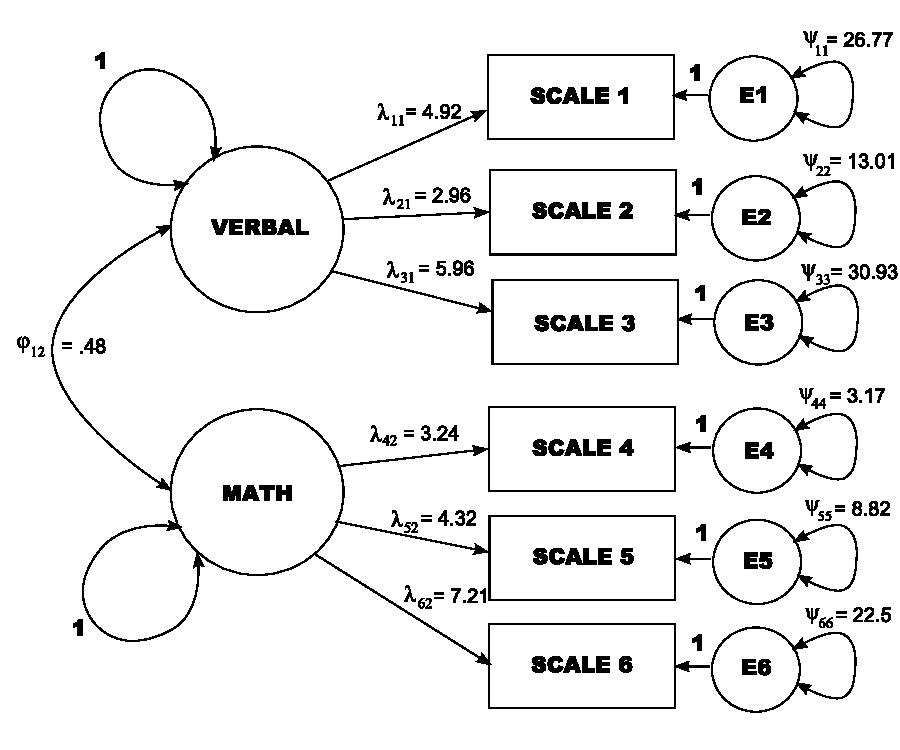
\includegraphics[height=5in]{famod.pdf}
%\input{figs/path}
\end{figure}


\section{Example with Artificial Data}

As an example of the ideas discussed above, consider a
hypothetical battery of six scales administered to students aged 13 to 18
years.  Three of the scales are intended to measure verbal ability, and
three of the scales are intended to measure mathematical ability.  We
may observe a maturation effect in the resulting data, whereby the scales
measure older students better than younger students (i.e., younger
students have not yet learned all the material).  The researcher's goal is to
study whether the scales are measurement invariant with
respect to age, which is taken to be the auxiliary variable $V$.

\subsection{Method}

To formally represent these ideas, we specify that the data arise from
a factor analysis model with two factors.  The base model, displayed in
Figure~\ref{fig:famod}, specifies that measurement invariance holds,
with three scales arising from the verbal factor and three 
scales arising from the mathematical factor.
For measurement invariance violations, we specify that $V$
(student age) impacts the values of 
verbal factor loadings in the model: 
if students are 16 through 18 years of age, then the factor
loadings corresponding to the first 
factor ($\lambda_{11}, \lambda_{21}, \lambda_{31}$) reflect those in
Figure~\ref{fig:famod}.  If students are 13 through 15 years of age,
however, then the factor loadings corresponding to the first factor
are three standard errors lower than those in Figure~\ref{fig:famod}
(the standard errors were obtained by fitting
  the model to a sample of size 200, where the sample consisted of all
  ``older'' subjects).
This violation states that the verbal ability scales
lack measurement invariance with respect to age.  For simplicity, we
assume that the mathematical scales are invariant.



A sample of size 200 was generated from the model described above, and
a test was conducted to examine measurement invariance of the three
verbal scales.  To carry out
the test, a confirmatory factor analysis model (with the paths
displayed in Figure~\ref{fig:famod}) was fit to the
data.  Casewise derivatives and 
the observed information matrix were then obtained, and they were used
to calculate the cumulative score process via
\eqref{eq:cumscore}.  Finally, we
obtained various test statistics and $p$-values from the cumulative score
process.  These include the double-max statistic from \eqref{eq:dmax},
the Cram\'{e}r-von Mises statistic from \eqref{eq:cvm}, and the max-LM
statistic from \eqref{eq:maxlm}.

Note that the tests give us the flexibility to test various subsets of
parameters.  For example, were we only interested in the 
three verbal factor loading parameters, we can test
\begin{equation}
    \label{eq:exh0}
H_0:\ (\lambda_{i,11}\ \lambda_{i,21}\ \lambda_{i,31}) =
(\lambda_{11}\ \lambda_{21}\ \lambda_{31}),\ i=1,\ldots,n,
\end{equation}
where $(\lambda_{i,11}\ \lambda_{i,21}\ \lambda_{i,31})$ represent the
verbal factor loading parameters for student $i$.  Alternatively, we
can consider all model parameters (including means), leading to a test
of \eqref{eq:h0}.  We consider both of these tests below.

\subsection{Results}
In the results section, we first describe overall results.  We then 
describe estimation of $\nu$, and 
isolation of model parameters violating
measurement invariance.  R code for obtaining these results is
  available at \url{http://semtools.r-forge.r-project.org}.

\subsubsection{Overall Results}
Test statistics for the hypotheses \eqref{eq:exh0} and~\eqref{eq:h0}
are displayed in  
Figure~\ref{fig:cusumex}.
Each panel displays a test 
statistic's fluctuation across values of student age, with the first
column containing tests of \eqref{eq:exh0} and the second column
containing tests of \eqref{eq:h0}.  The solid
horizontal 
lines represent critical values for $\alpha=.05$, and
the Cram\'{e}r-von Mises panels 
also contain a dashed line depicting the value of the test
statistic (test statistics for the others are simply 
the maxima of the processes).
In other words, for panels in the first and third rows, \eqref{eq:exh0} is
rejected if the process crosses the horizontal line.  For panels in
the second row, \eqref{eq:h0} is rejected if the dashed horizontal line is
higher than the solid horizontal line.

The figures display many test attributes, all of which generally
conform with the underlying theory.  First, when we test
only the three verbal factor loadings, all three tests can detect the
change.  Conversely, when all nineteen model parameters are tested,
only the double-max test detects a change.  This implies that 
power increases as larger proportions of tested parameters
change.  The results also imply that the double-max test is more
sensitive to fluctuations among a small subset of parameters.

Figure~\ref{fig:lrlm} 
compares the max-LM statistic (black line) to the max-LR
statistic (blue line) from \eqref{eq:maxlr}, as applied to testing
\eqref{eq:h0}.  The critical values for these two
tests are identical, hence the single horizontal line.
The figure
shows that the two statistics are very similar to one another, with
both maxima at the dotted vertical line.  This
is generally to be expected, because the two tests are asymptotically
equivalent.  For this specific situation, however, the max-LR
statistic rejects \eqref{eq:h0} while the max-LM statistic does not.
More generally, the 
max-LR statistic cannot be obtained from the empirical fluctuation
process, so it must be computed ``by hand'' (i.e., by computing
the LR statistic over all values of the threshold $\nu$, re-fitting the
factor analysis model for each value).

\subsubsection{Estimation of $\nu$ and Parameter Isolation}
As described above, the tests of \eqref{eq:exh0} imply that the 
verbal scales lack measurement invariance.  
We can also use the tests to: (1) estimate the 
threshold $\nu$, and (2) isolate specific parameters that violate
measurement invariance.  
For example, as described previously, estimates of $\nu$ can be obtained by
examining the peaks in Figure~\ref{fig:cusumex}.  For all six panels
in the figure, the peaks occur near an age of 16.1.  This agrees well
with the true threshold of 16.0.

The double-max test yields specific information about 
parameters violating measurement invariance.  Given
rejection of the hypothesis of measurement invariance \eqref{eq:exh0},
we can do posthoc 
tests to study specific parameters violating measurement invariance.
This involves individual examination of each parameter's cumulative
score process,
along with a procedure that controls for Type I error.  
Figure~\ref{fig:posthoc} shows the individual cumulative score processes for the
verbal factor loadings, with the horizontal lines reflecting the
critical value at $\alpha=.05$.
  The figure
shows that the third parameter (i.e., $\lambda_{31}$) crosses the
dashed line, so we would conclude a measurement 
invariance violation with respect to age for the third
verbal test.  The fact that the cumulative score process for the first
and second loadings did not achieve the critical value represents a Type II
error, which implicitly brings into question the posthoc tests' power.  We
generally address the issue of power in the simulations below.

\begin{figure}
\caption{Three test statistics of \eqref{eq:exh0} and \eqref{eq:h0}, 
  based on the example involving measurement invariance with respect
  to student age.  Solid, horizontal lines represent critical values
  at $\alpha=.05$, and the dotted, horizontal lines (second row)
  represent values of the Cram\'{e}r-von Mises test statistic.}
\label{fig:cusumex}
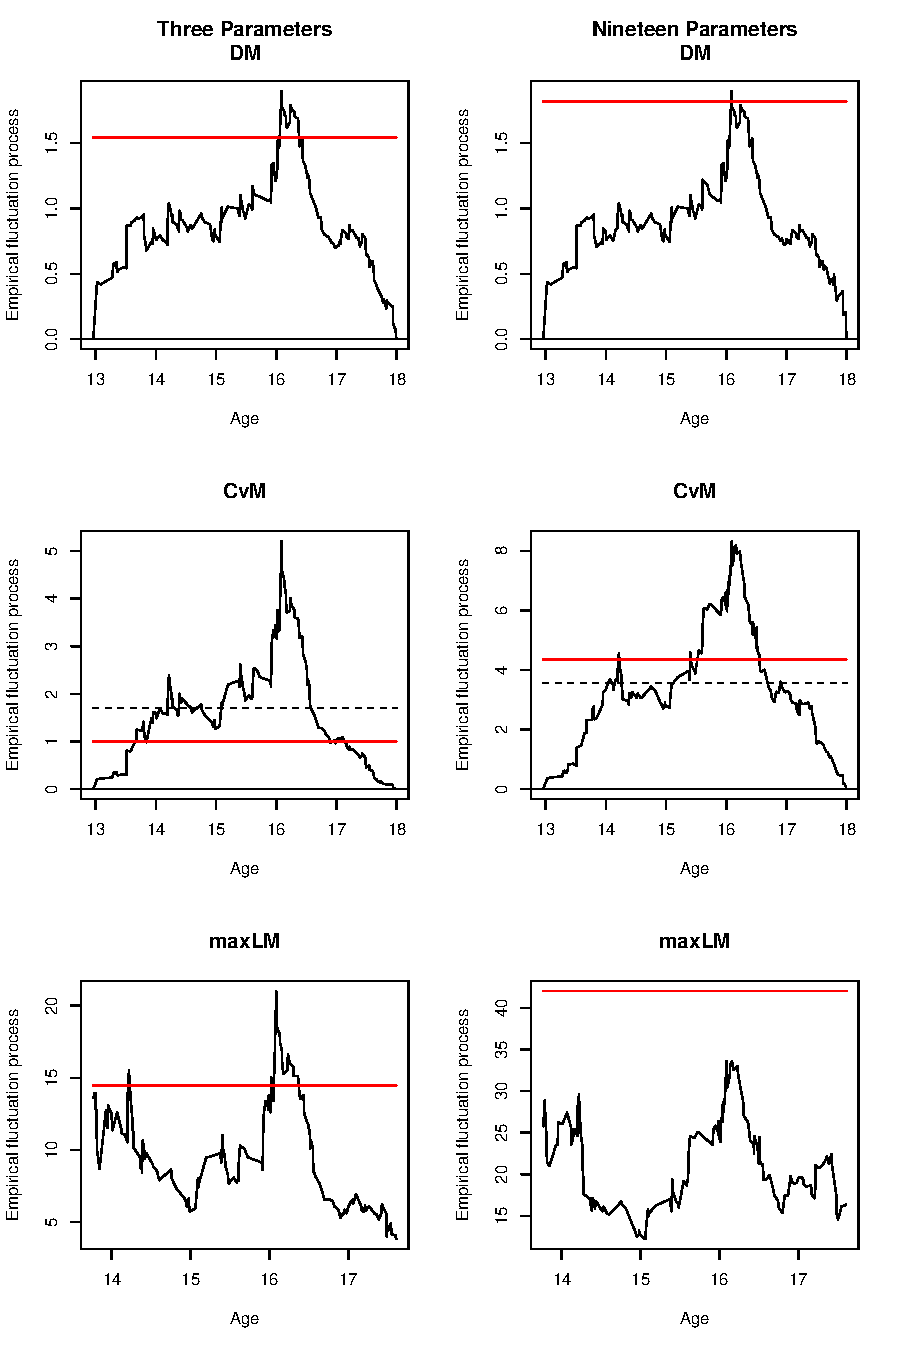
\includegraphics[height=9in]{gefp_3_19.pdf}
\end{figure}

\begin{figure}
\caption{A comparison of the max-LM (black line) and max-LR (blue line) test
  statistics for \eqref{eq:h0}.  The solid, horizontal line
  corresponds to the critical value at $\alpha=.05$.}
\label{fig:lrlm}
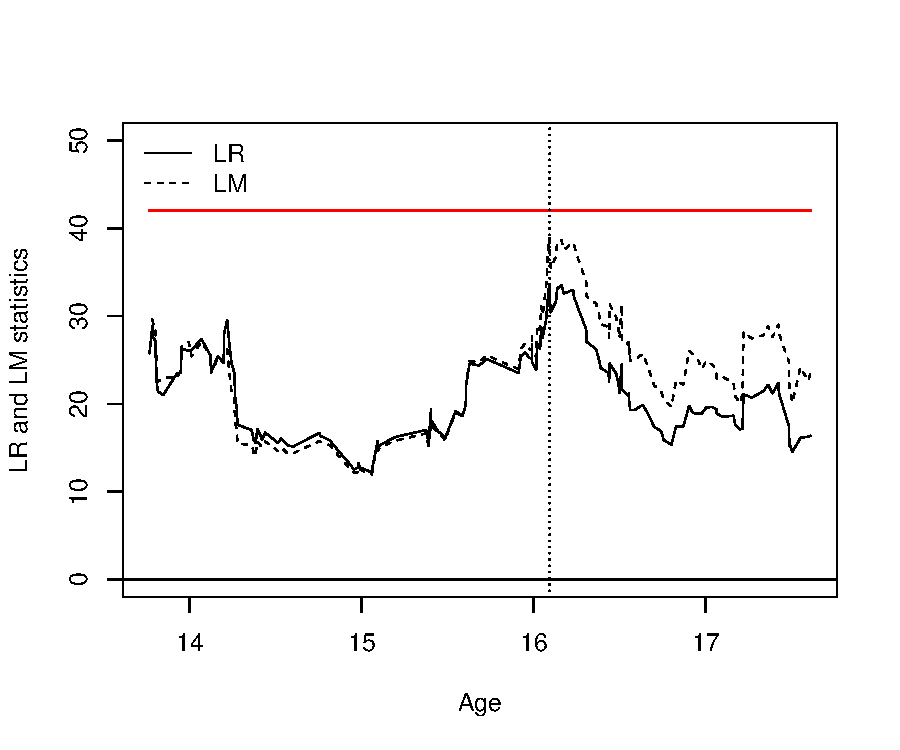
\includegraphics[height=5in]{lmlr_19.pdf}
\end{figure}

\begin{figure}
\caption{Posthoc tests of individual verbal factor loadings, based on
  the absolute maximum of each cumulative score process.  The top
  panel depicts the process for $\lambda_{11}$, the middle panel
  depicts the process for $\lambda_{21}$, and the bottom panel depicts
  the process for $\lambda_{31}$.  The solid, horizontal lines
  correspond to the critical value at $\alpha=.05$.}
\label{fig:posthoc}
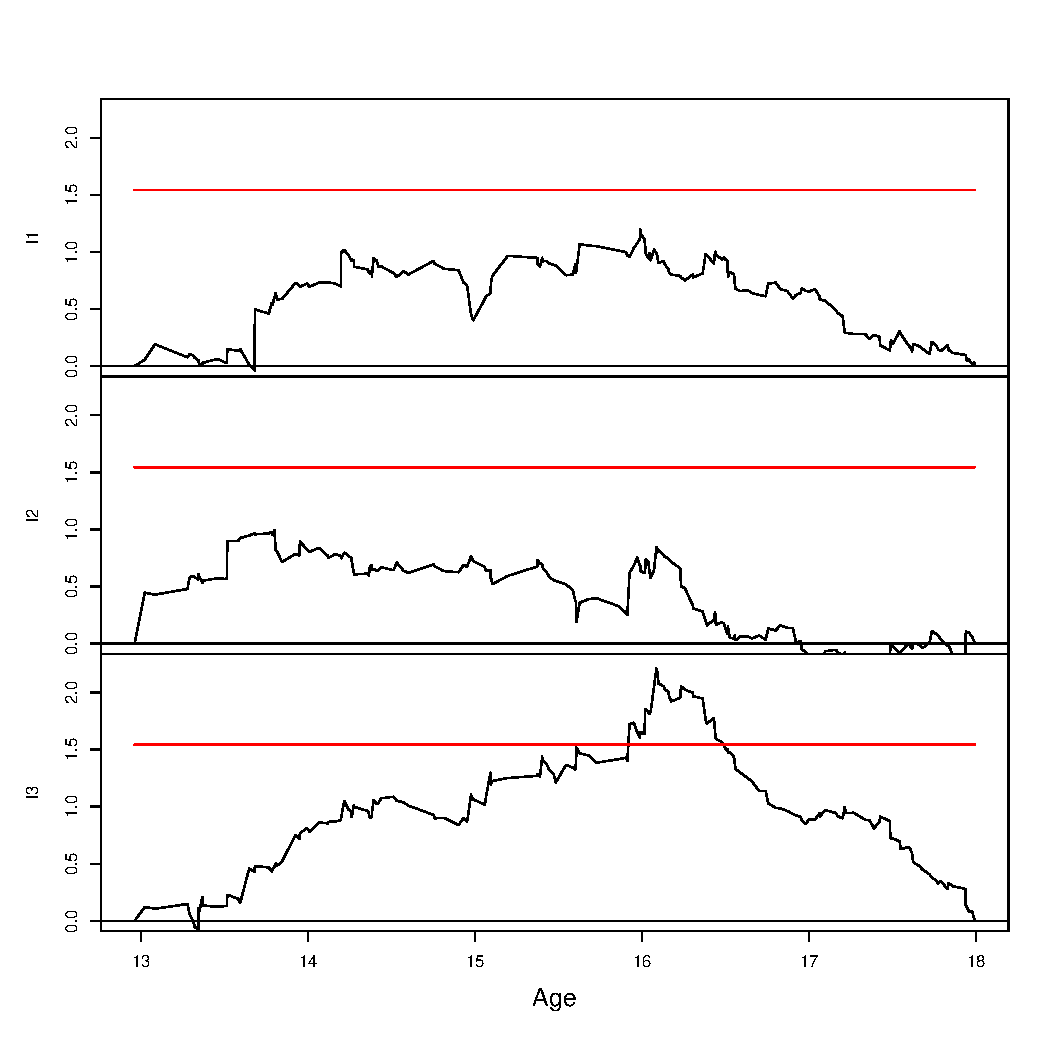
\includegraphics[height=5in]{gefp_posthoc.pdf}
\end{figure}

\section{Simulation}
% Simulations demonstrating power of test(s) at various
% sample sizes, types of invariance violations, ?
In this section, we conduct a simulation designed to
examine the tests' power and Type I error rates in a context
similar to the example.
We examine the power and error rates of three tests: the double-max test, the
Cram\'{e}r-von Mises test, and the max-LM test.  We also compare 
tests involving only the parameters that changed with tests of all model
parameters.  The example implied that the former tests had more
power, and the simulations provide more detail on the extent to which
power increases.  Finally, we also examine the tests' power across
various magnitudes of measurement invariance violations.

\subsection{Method}
Data were generated in a similar way to that of 
the Example section.
The data included verbal scales that violated measurement invariance
with respect to students' ages, with students 13--15 years of age
having smaller factor loadings than students 16--18 years of age.  
Simulation data were generated from the same general factor analysis
model (see Figure~\ref{fig:famod}), but sample size and magnitude
of measurement 
invariance violation were manipulated to examine power:
we examined power to detect 
invariance violations across three sample sizes ($n=100,
200, 500$) and three magnitudes of violations (factor loadings
for the younger students being $(0, 0.25, 0.5, \dots, 5)$ standard
errors\footnote{The standard errors used here were
  obtained by fitting
  the model to a sample of size 100, where the sample consisted of all
  ``older'' subjects.} below 
those for the older students).  The 0-standard error condition was
used to study Type I error rate.

\readme{Achim: Is it true that you used 5000 reps per cell?}
For each combination of sample size $\times$
violation magnitude $\times$ number of parameters being tested,
5,000 datasets were generated and tested.  In each dataset, half the
students were 13--15 
years of age and half were 16--18 years of age.

\subsection{Results}
Full simulation results are presented in Figure~\ref{fig:simres}, and
a subset of the results (for finer distinctions) is displayed in
Table~\ref{tab:simres}.  In describing the results, we largely refer
to the figure.

Figure~\ref{fig:simres} displays power as a function of violation
magnitude, with panels for each combination of sample size $\times$
number of parameters being tested.  
Circles reflect the double-max test, triangles reflect the max-LM
test, and plus signs reflect the Cram\`{e}r-von Mises test.  One can
generally observe that simultaneous tests of all 19 parameters
result in decreased power, with the tests performing very similarly at
the larger sample sizes.  The tests distinguish themselves from one
another when only the three factor loadings are tested, with the
Cram\`{e}r-von Mises test having the most power, followed by max-LM,
followed by the double-max test.  This advantage decreases with
increases in sample size.  
Absolute differences in power can be found in Table~\ref{tab:simres},
which contains a subset of the results.  For example, the table shows that the
power advantage of the Cram\`{e}r-von
Mises test can be as large as .1 (at $n=100$, 3 parameters being
tested).  It also shows that the Cram\`{e}r-von Mises test generally
has true Type-I error rates, with the double-max test being slightly
conservative and the max-LM test being slightly liberal at small
sample sizes.

In summary, we found that the proposed tests have adequate power to detect
measurement invariance violations in applied contexts.  The 
Cram\`{e}r-von Mises statistic exhibited the best performance for the
data generated here, though this result may not hold for all
situations.  In the discussion, we specifically consider the extent to 
which these findings may extend to other factor-analytic situations.

\begin{figure}
\caption{Simulated power for three test statistics across three sample
  sizes, two subsets of tested parameters, and measurement invariance
  violations of 0 to 5 standard 
  errors.  Circles reflect the double-max test, triangles reflect the
  max-LM test, and plus signs reflect the Cram\`{e}r-von Mises test.
  Numbers above each panel reflect the sample size and number of
  parameters being tested, respectively.}
\label{fig:simres}
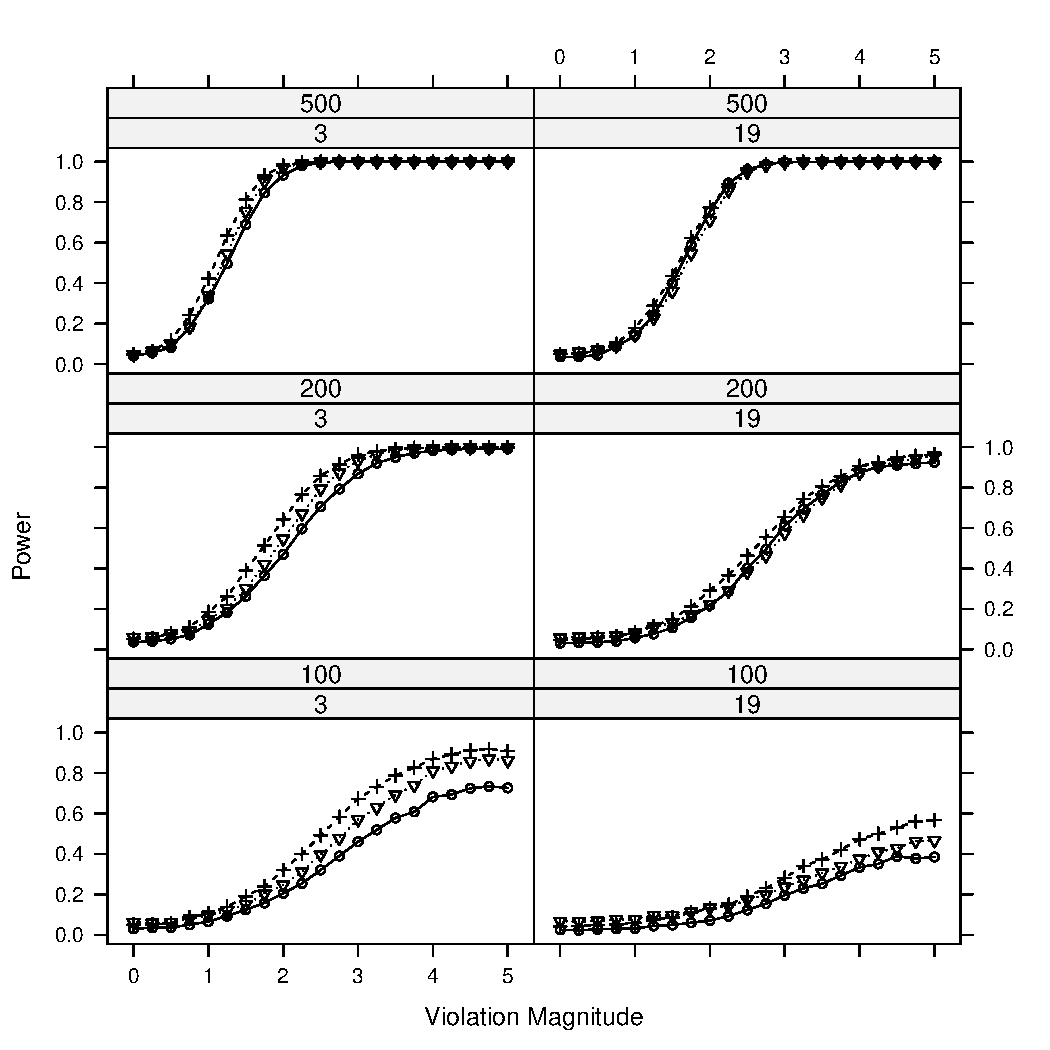
\includegraphics[height=5in]{simres.pdf}
\end{figure}


\begin{table*}
\caption{Simulated power for three test statistics
  across three sample sizes, eight magnitudes of measurement
  invariance violations, and two subsets of tested
  parameters. Abbreviations: CvM = Cram\'{e}r-von Mises 
  test; Max-LM = Maximum Lagrange multiplier test; DM = Double-max test.}
\label{tab:simres}
\begin{center}
\begin{tabular}{lllllllllll}
  \hline
   & & & \multicolumn{8}{l}{Violation Magnitude (SE)} \\
  $n$ &  npars &  Statistic    &  0 & 0.5 &    1 &  1.5
       &    2 &  2.5  &   3 &  3.5 \\ 
  \hline
  100  &  3    &  DM           &  3.1 &    3.6 &    6.6 &   12.4 &   20.6 &   32.1  &  46.1 &   57.8 \\ 
         &         &  CvM            &  5.0 &    5.7 &   10.6 &   19.1 &   32.1 &   49.2  &  67.2 &   78.8 \\ 
         &         &  max-LM          &  6.2 &    6.2 &    9.8 &   15.0 &   24.7 &   39.7  &  57.0 &   69.2 \\ 
         &  19   &  DM           &  2.5 &    2.8 &    3.1 &    4.9 &    7.1 &   12.4  &  19.6 &   25.3 \\ 
         &         &  CvM            &  4.2 &    4.8 &    5.8 &    8.6 &   13.0 &   18.9  &  28.2 &   37.4 \\ 
         &         &  max-LM          &  6.7 &    6.9 &    7.7 &    9.6 &   13.3 &   17.3  &  23.6 &   30.6 \\ 
  200  &  3    &  DM           &  3.7 &    5.2 &   12.5 &   26.3 &   47.0 &   70.6  &  86.8 &   95.0 \\ 
         &         &  CvM            &  5.3 &    7.9 &   18.6 &   39.1 &   64.3 &   85.8  &  96.2 &   99.0 \\ 
         &         &  max-LM          &  6.0 &    8.0 &   14.5 &   30.2 &   54.7 &   79.4  &  93.2 &   98.5 \\ 
         &  19   &  DM           &  3.2 &    3.6 &    5.7 &   10.8 &   21.9 &   40.2  &  61.1 &   76.5 \\ 
         &         &  CvM            &  4.6 &    5.8 &    8.5 &   15.0 &   29.1 &   46.4  &  65.4 &   80.7 \\ 
         &         &  max-LM          &  5.6 &    6.4 &    8.3 &   13.2 &   22.3 &   38.2  &  57.5 &   74.8 \\ 
  500  &  3    &  DM           &  4.1 &    8.3 &   32.2 &   69.0 &   93.4 &   99.5  & 100.0 &  100.0 \\ 
         &         &  CvM            &  4.7 &   11.8 &   42.2 &   81.3 &   98.0 &  100.0  & 100.0 &  100.0 \\ 
         &         &  max-LM          &  4.6 &    9.8 &   33.9 &   75.5 &   97.1 &  100.0  & 100.0 &  100.0 \\ 
         &  19   &  DM           &  3.6 &    4.4 &   14.0 &   40.1 &   75.3 &   96.0  &  99.7 &  100.0 \\ 
         &         &  CvM            &  5.0 &    6.7 &   17.9 &   43.6 &   77.4 &   95.9  &  99.7 &   99.9 \\ 
         &         &  max-LM          &  4.9 &    7.0 &   14.2 &   36.0 &   71.0 &   94.9  &  99.6 &  100.0 \\ 
   \hline
\end{tabular}
\end{center}
\end{table*}


\section{Discussion}
In this paper, we have presented a new family of statistical tests for
the study of measurement invariance in psychometrics.  The tests,
based on stochastic processes, have reasonable power, can isolate
groups of individuals violating measurement invariance based on a
continuous, auxiliary variable, and can
isolate specific model parameters affected by the violation.  In this
section, we consider the tests' use in practice and their 
extension to more complex scenarios.

\subsection{Use in Practice}
% Simultaneous test of Meredith's various types of invariance
The proposed tests give researchers a new set of tools for studying 
measurement invariance.  For example, they give researchers the
flexibility to: (1) simultaneously test all model parameters, yielding
results relevant to many types of measurement
invariance (see, e.g., \citeNP{Mer93}), or (2) test a single subset of
model parameters, potentially leading to improved power to detect a
single type of measurement invariance.  The traditional
steps have involved hypothesizing a specific type of invariance and
then testing for it via a Likelihood Ratio Test, but this is
unnecessary under the proposed framework.

% Researchers interpreting subgroups violating MI
In addition to simultaneously testing different types of measurement
invariance, the proposed tests allow researchers to easily interpret
the nature of the invariance violation.  This is made possible through
the tests' abilities to estimate $\nu$, the threshold dividing
individuals into subgroups that violate
measurement invariance.  While a single $\nu$ was assumed in this
paper, it is also possible to define 
formal rules for estimating multiple $\nu$ parameters.  We plan to
explore these ideas in the future.

% \subsection{Further Issues}
% Further issues associated with the proposed tests include: (1)
% alternative methods for estimating $\eta$;
% and (2) dealing
% with categorical $V$.  We address each in turn below. 

% % More than two groups violating MI
% \subsubsection{Estimation of $\eta$}
% Given rejection of the hypothesis of measurement invariance, the most
% straightforward way to formally estimate $\eta$ is through
% the location of the maximum of the cumulative score process.  Assuming
% a single threshold, the maximum should be achieved close to the true
% $\eta$.  Referring to the Example (see
% Figure~\ref{fig:cusumex}), we defined $\eta$ as the 
% age corresponding to the solid dot in the third panel.

% To study this method in more detail, we used
% results of our simulation to examine the age at which the maximum of
% the cumulative score process occurs.
% If the test accurately recovers the violating subgroups,
% then the maximum should be close to 16 years
% of age.\footnote{The data generated for these
%   simulations 
%   contained ages measured in days, as opposed to years.  Thus,
%   the tests could split students at continuous values like 15.6 or
%   16.3 years of age.}
%   For each simulation condition, Table~\ref{tab:age1}
%   displays confidence intervals for the location of the maximum
%   absolute cumulative score.  These confidence intervals were
%   calculated across generated 
%   datasets, with each dataset contributing one maximum absolute cumulative
%   score
%   (regardless of whether the hypothesis of
%   measurement invariance was rejected).
% It is observed that these confidence intervals slightly underestimate
% the true age dividing the subgroups, with the degree of bias
% decreasing as sample size increases.  The interval widths
% are impacted by both the magnitude of the invariance and the sample
% size.  In future work, we plan to study alternative ways of
% identifying subgroups.

% \begin{table*}
% \caption{Confidence intervals for the location of the maximum absolute
%   cumulative score across the conditions from the simulation.}
% \label{tab:age1}
%   \begin{tabular}{lccc} \thickline
%   & \multicolumn{3}{c}{Violation Magnitude} \\
%   $n$ & 1SE & 2SE & 3SE \\\hline
%   100 & (15.61; 15.73) & (15.55; 15.65) & (15.50; 15.59) \\
%   200 & (15.67; 15.77) & (15.64; 15.72) & (15.67; 15.73) \\
%   500 & (15.71; 15.81) & (15.77; 15.83) & (15.80; 15.83) \\\thickline
%   \end{tabular}
% \end{table*}

% Differing proportions of people in each group
%\subsubsection{Subgroup Proportions}
%The power of the proposed tests is impacted by the proportion of
%individuals within each subgroup.  

% Ties on auxiliary variable (mention use in categorical contexts)
\subsection{Categorical Auxiliary Variable}
% There remain unaddressed theoretical issues specific to the 
% tests' application to measurement invariance.  These
% issues generally stem from the types of auxiliary variables on which
% researchers may study measurement invariance.  In
% the example described earlier, researchers wanted to know whether a
% scale was measurement invariant with respect to student age.
% Students could then be ordered based on age, and a test could be 
% constructed via Equation~\eqref{eq:cumscore}.  However, an issue arises if there
% are ties on age; that is, if two students' ages are exactly
% the same.  The proposed tests assume complete ordering of the
% students, but these two students cannot be ordered.  In this case, we
% may randomly order the two students, but there is an
% arbitrariness associated with this strategy.  Alternatively, to obtain
% tests that liberally reject the hypothesis of measurement invariance,
% we may choose the ordering that results in the largest test
% statistic.  If there are many tied students, then there are many
% possible orderings that must be examined.  However, examination of all
% possible orderings remains computationally feasible because the
% casewise first derivatives need to be calculated only once; the
% derivatives simply need to be reordered for each ordering of tied
% students.

One issue that was largely unaddressed in this paper involved the use
of categorical $V$ to study measurement invariance.  In this case,
groups are 
already specified in advance, and so traditional methods (i.e.,
Likelihood Ratio tests) may suffice.
However, we could use the framework developed here to obtain an
alternative $\chi^2$ statistic testing measurement invariance.
Assume the observations are divided into $K$ categories $I_1, I_2,
\ldots, I_K$.
First, we can sum scores within each category of the
demographic variable via:
\begin{equation}
    \label{eq:catsum}
    \Delta W_n(I_k) = \frac{1}{n_k\sqrt{n}} \sum_{i \in I_k}
    {\bm{I}}(\widehat{\bm{\theta}})^{-1/2} {\bm{\psi}}({\bm{y}}_i, \widehat{{\bm
      \theta}}),
\end{equation}
where $n_k$ is the sample size in category $k$ and $n$ is the overall
sample size.  This results in a $K \times p$ matrix, with one entry for
each category-by-model parameter combination.  We can test
a specific model parameter for invariance by focusing on the associated
column of the $K \times p$ matrix, summing over the squared entries in
the column to obtain a $\chi^2$-distributed statistic with
$(K-1)$ degrees of freedom \cite{HjoKon02}.
Alternatively, to simultaneously test multiple parameters, we can sum
the $\chi^2$ statistics and degrees of freedom for the individual
parameters.

\subsection{Extensions}
The proposed family of tests can be extended in various ways.  First,
it is possible to construct an algorithm that recursively defines
groups of individuals violating measurement invariance with respect to
multiple auxiliary variables.  Such an algorithm is related to 
classification and regression trees \cite{BreFri84,MerSha10,StrMal09},
with related algorithms being developed for generalized linear
models \cite{ZeiHot08} and Rasch models \cite{KopZei10}.  

Relatedly,
S\'{a}nchez \citeyear{San09} described a general
method for partitioning/segmenting structural equation models within a 
partial least squares framework.  This method involves direct maximization of
the likelihood ratio (i.e., fitting the model for various subgroups
defined by 
$V$ and choosing the subgroups with the largest likelihood ratio),
however, instead of the tests described in this paper.  The tests
described here are highly advantageous because they only require the
model to be estimated once.

% Recursive method
% \subsubsection{Recursive Multiple-Groups Models}
% The proposed tests have the ability to automatically define groups of
% individuals violating measurement invariance with respect to a single
% auxiliary (often demographic) variable.  If a researcher has multiple
% auxiliary variables that he/she wishes to assess for measurement
% invariance, then the proposed tests can be inserted into a recursive
% algorithm 
% that isolates groups of individuals violating measurement
% invariance.   and
% C4.5 \cite{Qui93}.  The algorithm would proceed via the following
% steps: 
% \begin{enumerate}
%   \item Fit a confirmatory factor analysis model to the data, with all
%   parameters constrained to be equal across observations.
%   \item Conduct a measurement invariance test with respect to each
%     auxiliary variable (auxiliary variables are determined in
%     advance by the researcher).
%   \item If violations of measurement invariance are detected,
%   split the data into two (or more) groups based on the auxiliary variable
%     corresponding to the largest test statistic.
%   \item Fit a multiple-groups factor analysis model based on step 3.
%   \item Repeat steps 2--5.
% \end{enumerate}
% The algorithm would continue until it reaches a
% predefined stopping rule.  For example, we may stop 
% the algorithm when the tests fail to indicate measurement invariance
% violations.  Alternatively, the algorithm may be stopped when the
% sample size within any subgroup reaches a minimum level.

% The algorithm described in the previous paragraph is related to one
% developed by Zeileis et al.\ \citeyear{ZeiHot08} for representing
% parameter invariance violations in generalized linear models.  Zeileis
% et al.\ present the results in a tree structure, which is
% suboptimal for factor analysis models.  Instead, the subgroups
% discovered by the algorithm are used here to adaptively define a
% multiple-groups factor analysis model.  The
% simultaneous study of measurement invariance with respect to multiple
% auxiliary variables is an important future direction.

%\subsubsection{Other Latent Variable Models}
Aside from recursive measurement invariance detection, the proposed tests
readily extend to other popular psychometric models.  
Instead of studying measurement invariance in factor
analysis, the tests can be used to generally 
study the stability of structural equation model parameters across
observations.  For 
example, it would be possible to assess whether relationships between
latent variables are stronger for some students than for
others.  Secondly, 
the tests may be extended to study differential item functioning (DIF)
in item response models (e.g., \citeNP{KopZei10}, who focused on an
application to Rasch models).  
DIF methods are similar to those for factor analysis in
that subgroups must be specified in advance.  The tests proposed here
can detect subgroups automatically, however, offering a unified way of
studying both 
measurement invariance in factor analysis and differential item
functioning in item response.  While these
two methods have developed largely independently of one another,
some treatments \cite{Mcd99} and recent research \cite{StaChe06} have
sought to unify the methods.  Extensions of the proposed tests can
support this endeavor.

\subsection{Summary}
We have outlined a family of 
stochastic process-based parameter instability tests from theoretical
statistics to the issue of measurement invariance in psychometrics.
The paper included both theoretical development and 
study of the tests' performance.  The tests were found via simulation
to have good properties, making them useful for many psychometric
applications.  More generally, the tests help to
solve standing problems in
measurement invariance research and provide many avenues for
future research, both through extensions of the tests within a
factor-analytic context and through application of the tests to new
models.

\bibliography{list}

\end{document}